
% This LaTeX was auto-generated from MATLAB code.
% To make changes, update the MATLAB code and republish this document.

\documentclass{article}
\usepackage{graphicx}
\usepackage{color}

\sloppy
\definecolor{lightgray}{gray}{0.5}
\setlength{\parindent}{0pt}

\begin{document}

    
    
\section*{Task 1}

\begin{par}
Analysis of non-linear and linearized water tank model with and without PID control.
\end{par} \vspace{1em}

\subsection*{Contents}

\begin{itemize}
\setlength{\itemsep}{-1ex}
   \item Model and linearization
   \item State Space Representation
   \item Simulation of open loop system
   \item Transfer function response
   \item Step response with control
   \item Applying the control to the non-linear and linearized plants in simulink
\end{itemize}


\subsection*{Model and linearization}

\begin{par}
Differential equation describing the tank water level:
\end{par} \vspace{1em}
\begin{par}
$$ \frac{d}{dt}H = \frac{bV-a\sqrt{H}}{A} $$
\end{par} \vspace{1em}
\begin{par}
This ode is non-linear in \ensuremath{\backslash}sqrt\{H\}. However, we can approximate this by a first order taylor expansion/linearization:
\end{par} \vspace{1em}
\begin{par}
$$ \sqrt{H_0 + \hat{H}} = \sqrt{H_0} + \frac{1}{2\sqrt{H_0}}\cdot (H-H_o) $$
\end{par} \vspace{1em}
\begin{par}
With this linearization we arrive at the linear ODE:
\end{par} \vspace{1em}
\begin{par}
$$ \frac{dH}{dt} =\frac{b}{A} V - \frac{a}{2A} \sqrt{H_0} (H-H_0) - \frac{a\sqrt{H_0}}{A} $$
\end{par} \vspace{1em}


\subsection*{State Space Representation}

\begin{par}
We can find the state space representation of this system (ignoring the non-homogeneous part):
\end{par} \vspace{1em}
\begin{par}
$$ \frac{d}{dt} H = \left[\matrix{ - \frac{a}{2A \sqrt{H_0}}} \right] H + \left[\matrix{ \frac{b}{A}} \right]V $$
\end{par} \vspace{1em}
\begin{par}
Alternatively, with our constants and linearization point:
\end{par} \vspace{1em}
\begin{par}
$$ \dot{H} = \left[\matrix{ - \frac{3\sqrt{10}}{80}} \right] H + \left[\matrix{ \frac{1}{3}} \right]V $$
\end{par} \vspace{1em}
\begin{par}
Our state space consists of a one-dimensional state vector H and a one-dimensional control vector V
\end{par} \vspace{1em}


\subsection*{Simulation of open loop system}

\begin{par}
For fun, we can simulate the non-linear and linearized differential equations to inspect the accuracy To do this I use matlab's ode45 which can simulate most ordinary differential equations The non-linear and linear ODE's are defined in tank\_system\_linear.m and tank\_system\_nonlinear.m, respectively.
\end{par} \vspace{1em}
\begin{verbatim}
A = 24; b = 8; a = 18; %water tank parameters

timespan = [0, 80]; %simulaion interval
H0 = 10; %initial level
colormap = turbo(11);

% Solve the and plot the ODE's
figure;
hold on;
for V = 0:10
    [t, H] = ode45(@(t, H) tank_system_nonlinear(t, H, a, b, A, V), timespan, H0);
    plot(t, H, 'Color', colormap(V+1, :));

    [t, H] = ode45(@(t, H) tank_system_linear(t, H, a, b, A, V, H0), timespan, H0);
    plot(t, H,'--','Color', colormap(V+1, :));
end

xlim(timespan);       ylim([0,20]);
xlabel('Time (s)');   ylabel('Height (H)');
title('Non-linear (solid) vs linearized (stippled)');
\end{verbatim}

        \color{lightgray} \begin{verbatim}Warning: Imaginary parts of complex X and/or Y arguments ignored. 
\end{verbatim} \color{black}
    
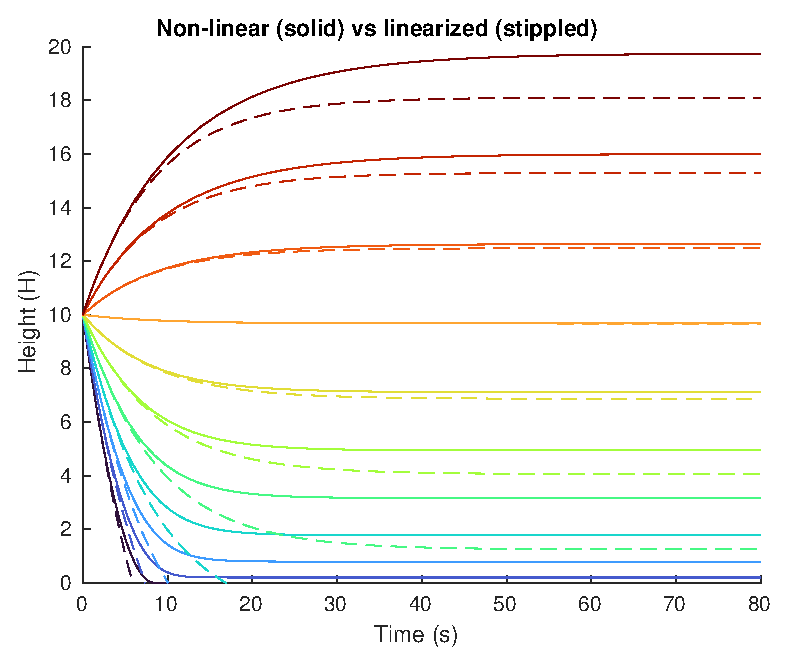
\includegraphics [width=4in]{main_01.eps}


\subsection*{Transfer function response}

\begin{par}
The transfer function is determined by taking the laplace transform of the homogeneous linear ODE:
\end{par} \vspace{1em}
\begin{par}
$$ \frac{H(s)}{V(s)} = \frac{\frac{b}{A}}{s+0.16\frac{a}{A}}$$
\end{par} \vspace{1em}
\begin{par}
Here, I simulate and plot the closd loop step responses for varying proportional gains:
\end{par} \vspace{1em}
\begin{verbatim}
close;

H0 = 0; %initial tank level
V = 1; %step response no feedback
H_desired = 1; %setpoint
colormap = turbo(11);

step_timespan = [0, 5];
figure;
grid on;
hold on;

%without feedback:
Kp = 0;
[t, H] = ode45(@(t, H) tank_system_step(t, H, a, b, A, H_desired, H0, V), timespan, H0);
plot(t, H, 'Color', 'k', 'LineWidth', 2, 'DisplayName', 'No Feedback');

for i = 0:10
    Kp = i*1.5;
    [t, H] = ode45(@(t, H) tank_system_step_feedback(t, H, a, b, A, H_desired, H0, Kp), timespan, H0);
    plot(t, H, 'Color', colormap(i+1, :), 'DisplayName', sprintf('Kp = %d', Kp));
end

xlim(step_timespan);       ylim([0,3]);
xlabel('Time (s)');   ylabel('Height (H)');
legend('Location', 'northwest');
\end{verbatim}

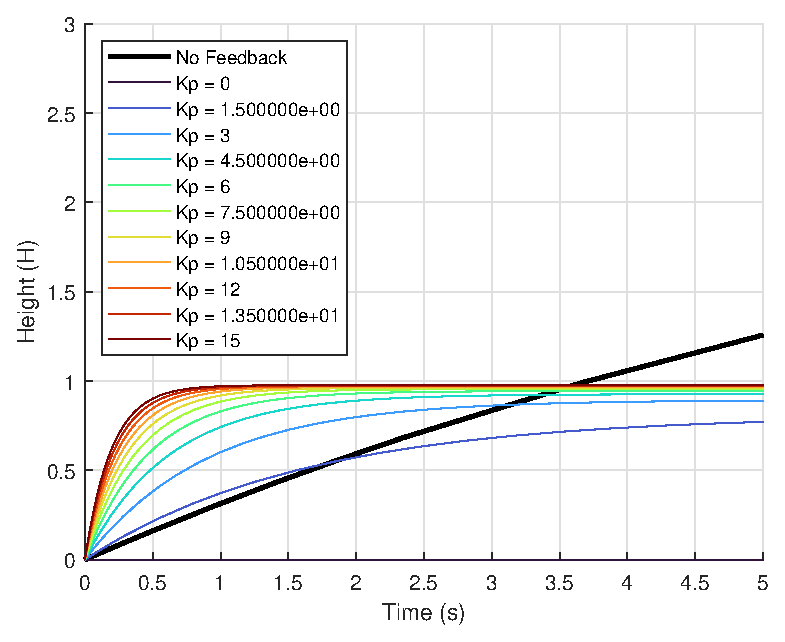
\includegraphics [width=4in]{main_02.eps}
\begin{par}
Since the system is a first-order linear system without disturbances, it behaves nicely and doesn't reach any oscillations.
\end{par} \vspace{1em}


\subsection*{Step response with control}

\begin{par}
Now we develop a complete PID controller for our plant using the transfer function of the linearized model.
\end{par} \vspace{1em}
\begin{verbatim}
close;
s = tf('s');

A = 24; b = 8; a = 18; %water tank parameters
tf_linear = (b/A)/(s+1/(2*sqrt(10))*(a/A)); %defining transfer function as given in the task
step(tf_linear);
\end{verbatim}

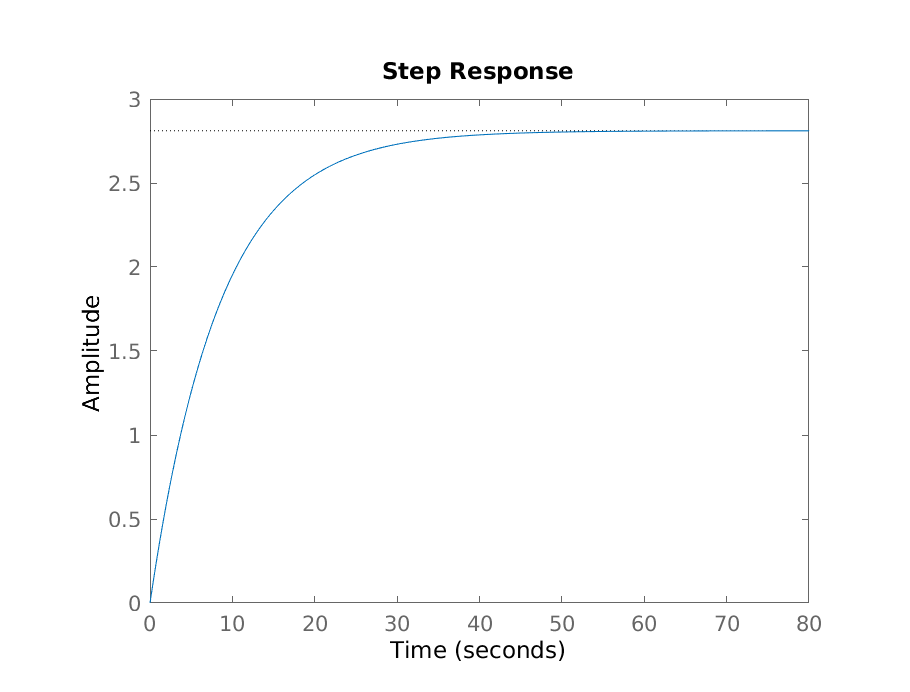
\includegraphics [width=4in]{main_03.eps}
\begin{par}
Now we tune all the gains to achieve the desired response
\end{par} \vspace{1em}
\begin{verbatim}
Kp = 15;
Ki = 5;
Kd = 1;

H = tf_linear; %plant transfer function
C = Kp + Ki/s + Kd*s; %PID transfer function

CH = C*H; %closed loop transfer function
closed_tf = CH/(CH+1);
step(closed_tf);

info = stepinfo(closed_tf);
overshoot     = info.Overshoot;
rise_time     = info.RiseTime;
settling_time = info.SettlingTime;

% Display results
fprintf('Overshoot: %.2f%%\n', overshoot);
fprintf('Rise Time: %.2f s\n', rise_time);
fprintf('Settling Time: %.2f s\n', settling_time);
grid on;
\end{verbatim}

        \color{lightgray} \begin{verbatim}Overshoot: 2.95%
Rise Time: 0.49 s
Settling Time: 2.95 s
\end{verbatim} \color{black}
    
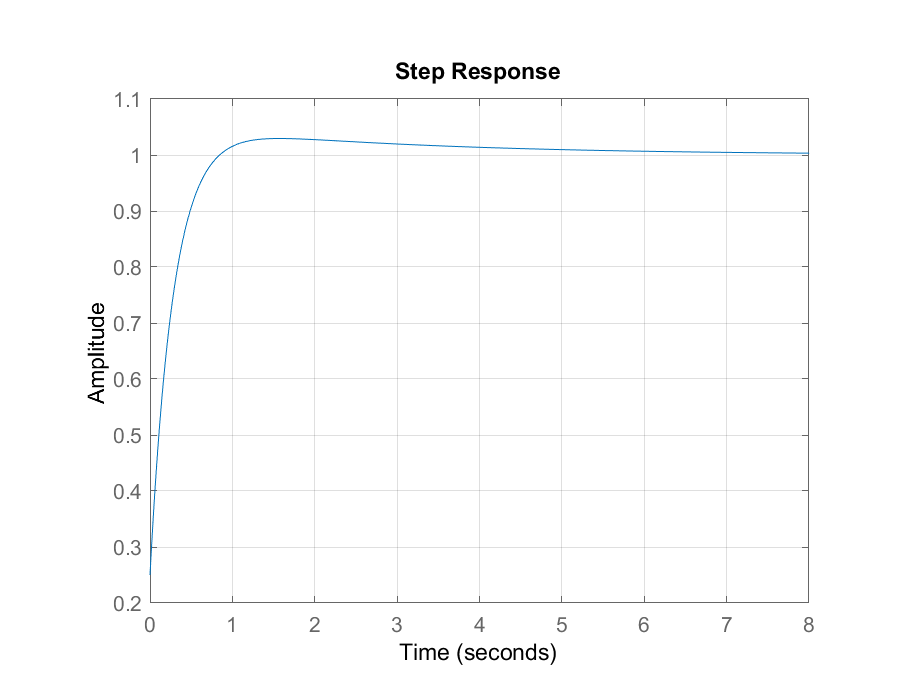
\includegraphics [width=4in]{main_04.eps}


\subsection*{Applying the control to the non-linear and linearized plants in simulink}

\begin{par}
With our conservative gains [Kp, Ki, Kd] = [15, 5, 1] We achieved a nice response.
\end{par} \vspace{1em}
\begin{par}
Now, I plot the response for a setpoint of 10 an an initial tank level of 9, for both the non-linear and linear systems.
\end{par} \vspace{1em}
\begin{par}
See simulink scope plots!
\end{par} \vspace{1em}



\end{document}

